\chapter{Context Transformation: Selection, Compaction, and Policy-Controlled Editing}\label{ch:C12}

The October 2026 transparent-compaction implementation preserves conversational prose while masking recoverable blocks and exposing delegated lookup; Context Language Models instead permit programmatic edits to the live context~\cite{woolford2026transparent,shao2026context}. These mechanisms alter different information and execution boundaries. Comparing them requires a transformation contract, downstream continuation loss, restoration cost, and an exact record of which view conditioned each action.

\section{The working view as a controlled variable}\label{sec:C12:control}
Context engineering is the construction of the actual conditional input on which a policy selects its next action. It includes the selection of instructions, evidence, tool descriptions, intermediate results, and unresolved commitments. Compaction is one intervention within that broader process. An agent can compact history while preserving raw storage, evict a cache without editing text, or edit its visible history without deleting a persistent record. These operations affect different state variables and should have different names in an implementation.

Let $H_t$ denote the append-only interaction evidence, $M_t$ the persistent memory, and $\mathcal C_t$ the model's working context. A context controller chooses an editing action $u_t$ before the task policy chooses an environment action $a_t$:
\begin{align}
 \mathcal C_t&=g(H_t,M_t,u_t),\\
 a_t&\sim\pi_\theta(\cdot\mid\mathcal C_t),\\
 u_t&\sim\mu_\psi(\cdot\mid H_t,M_t,B_t).
\end{align}
Here $B_t$ is the remaining resource budget. The decomposition can be implemented by separate models, one model with distinct action types, or deterministic harness logic. It is a functional distinction, not a claim that a separate context model is always beneficial. Access to $H_t$ is not free: the total account must charge the controller's scans, retrieval, model calls, and storage operations as well as the task policy's input.

The context controller faces an unusual delayed-control problem. Removing a record can make the next request cheaper but create a failure many steps later. Its reward is mediated by another policy and by the environment. A controller trained only to reduce input size may learn aggressive deletion that looks efficient until a deferred constraint becomes decisive. Conversely, penalizing every retrieval call can encourage a policy to retain large amounts of irrelevant content. The objective must include task outcome and complete lifecycle cost.

A useful constrained formulation uses a total resource cost $C_{\mathrm{total}}$, a terminal success indicator $Y_s\in\{0,1\}$, and an indicator $Y_u\in\{0,1\}$ that at least one unauthorized effect occurred. For fixed task and environment distributions, define
\begin{equation}
 \min_{\mu,\pi}\mathbb E[C_{\mathrm{total}}]
 \quad\text{subject to}\quad
 P_{\mu,\pi}(Y_s=1)\geq\tau,
 \quad P_{\mu,\pi}(Y_u=1)\leq\delta.
\end{equation}
The thresholds $\tau,\delta\in[0,1]$ are workload-specific requirements. They are not established constants, and success estimation must retain failures and timeouts. A Lagrangian objective can aid optimization, but it does not prove that the constraints hold after training. Authorization should generally be enforced outside a stochastic controller rather than represented only as a reward penalty.

The central design question is which distinctions the working view must preserve. A context assembled for code editing needs current files, interface constraints, test outcomes, and rejected hypotheses. A literature agent needs claims, supporting passages, conflicting evidence, and unresolved source identities. Applying the same generic summary template to both workloads can remove the information that makes their next actions valid. State fields should follow decision requirements, with prose used where a schema would erase necessary nuance.


\section{Selection before abstraction}\label{sec:C12:selection}
Selection retains some records verbatim; abstraction constructs a new record that represents several old ones. These operations have different error modes. Selection can omit a decisive source while faithfully preserving everything selected. Abstraction can include the right sources but misstate their contents, merge incompatible claims, or remove a qualification. A practical pipeline should make the two stages separately inspectable instead of treating a single generated summary as an opaque transformation.

Suppose records $r_i$ have token costs $c_i$, and $F(S)$ is the task-dependent utility of retaining the records indexed by $S$. A simple selection model is a budgeted set problem:
\begin{equation}
 \max_{S\subseteq\{1,\ldots,n\}}F(S)
 \quad\text{subject to}\quad\sum_{i\in S}c_i\leq W.
\end{equation}
If $F$ is monotone submodular, marginal-gain heuristics have useful theoretical properties under suitable assumptions. Agent evidence does not generally satisfy those assumptions. Two individually useless records can jointly identify a contradiction, while one new correction can invalidate many older records. Utility may be complementary or nonmonotone. Using a greedy score can still be an engineering heuristic, but its approximation guarantees do not transfer without verifying the required structure.

Abstraction introduces a different optimization target. Let $z=s(R)$ be a summary of records $R$ and let $\mathcal D_R$ be a specified conditional distribution over future requests $q$ and targets $Y$ given that source record. Define distortion through paired decision losses rather than textual similarity:
\begin{equation}
 d(R,z)=\mathbb E_{(q,Y)\sim\mathcal D_R}
 \left[\ell\{\pi(q,z),Y\}-\ell\{\pi(q,R),Y\}\right].
\end{equation}
This is a proposed operational distortion measure. Both conditions receive the same request--target draw; a stochastic policy's internal sampling is also included in the expectation. The controller observes $R$ and the current request, not the evaluation target $Y$. Distortion can be negative when abstraction removes distraction, and it depends on the evaluated policy. It is not a mathematical distance. Holding $\mathcal D_R$ fixed prevents a change in the future-question distribution from being misreported as better preservation.

Preserving exact text is especially valuable for identifiers, numeric requirements, authorization, and claims requiring attribution. A summary may safely paraphrase a search strategy while retaining an exact test failure or contract clause as a quoted evidence object. The representation can combine concise state with evidence pointers rather than forcing every item into the same compression format. Token allocation should reflect the cost of a mistaken abstraction, not only the record's length.

An implementation can maintain an immutable source layer, a typed decision-state layer, and a generated narrative layer. Each narrative assertion should link to one or more source objects or be marked as an inference. Contradictions remain separate objects until resolved by an explicit rule. This architecture makes it possible to regenerate a summary after a correction without pretending that the first summary was an authoritative replacement for the evidence.


\section{Reversible offload and explicit context actions}\label{sec:C12:offload}
ACM makes context management an explicit part of agent behavior through a summarization action and retrieval of earlier raw interaction history~\cite{corpus260723809}. Its distinction between a bounded active view and preserved external history is technically important. Offloaded text can remain intact while the working context becomes lossy. The agent still has to recognize when it needs an omitted detail, issue a suitable retrieval request, and interpret the returned record correctly. Storage reversibility and behavioral reversibility are different properties.

The paper's mechanism can be understood as a state transition with a retained suffix, a compacted prefix, and access to raw evidence. The resulting policy is more flexible than mandatory truncation at a fixed threshold because it can choose when to summarize. That flexibility creates a larger action space and additional credit-assignment demands. The context-management decision can be correct locally but harmful to a later step, so evaluating only the immediate post-summary answer is insufficient.

Context Language Models go further by making the live context directly editable and studying serving support for such edits~\cite{shao2026context}. Their reported FLOP accounting should not be equated with measured latency or service expenditure. The generalizable distinction is between a fixed set of harness editing operations and a model-controlled editing program. The latter expands expressivity but also expands the space of invalid or semantically damaging edits.

A conservative editing interface can represent operations as typed transformations: retain, summarize, externalize, restore, annotate, and invalidate. Each operation has preconditions and a provenance record. ``Invalidate'' should preserve the reason a fact became obsolete; it should not silently erase the record needed to understand a past decision. ``Restore'' should recover source roles and timestamps together with text. A raw paragraph returned without its original authority can change its meaning.

The proposed construction below is an implementation contract, not a reproduction of ACM's code. Let $R=\mathcal P(S)$ pin obligations and authority-bearing records from state $S$, $D=\mathcal L(H,S)$ locate a finite set of currently readable candidate evidence in history $H$, and $N=\mathcal N(H,S)$ retain recent events. The token-cost map $\ell$ measures the variable serialization charge against residual capacity $W$; fixed material already reserved in $W$ is not charged again. When $\ell(R)\leq W$, a declared selector $\sigma$ chooses from
\begin{equation}
\begin{aligned}
 \mathfrak E_W
   &=\left\{E\subseteq D:
      \ell(R)+\sum_{r\in E}\ell(r)\leq W\right\},\\
 E_W&=\sigma(\mathfrak E_W;H,S),\\
 z_W&=\mathcal S(E_W),\qquad
 c_W=\Sigma(R,z_W,N).
\end{aligned}
\label{eq:C12:context-construction}
\end{equation}
Here $\mathcal S$ summarizes with source identifiers and $\Sigma$ serializes the pinned records, summary, and recent events. No optimality of $\sigma$ or semantic sufficiency of $\mathcal S$ is assumed. Let $v(R,c_W)\in\{0,1\}$ test structural preservation of the pinned records in the completed serialization. A conservative admissibility rule returns either the completed context, an infeasible-budget marker $\bot_B$, or a failed-preservation marker $\bot_V$:
\begin{equation}
 \widehat C_W=
 \begin{cases}
 \bot_V,&v(R,c_W)=0,\\
 \bot_B,&v(R,c_W)=1,\ \ell(c_W)>W,\\
 c_W,&v(R,c_W)=1,\ \ell(c_W)\leq W.
 \end{cases}
\label{eq:C12:context-admissibility}
\end{equation}
This inner construction is defined only when $\ell(R)\leq W$. The complete budget guard is
\begin{equation}
 C_W=
 \begin{cases}
 \bot_B,&\ell(R)>W,\\
 \widehat C_W,&\ell(R)\leq W.
 \end{cases}
\label{eq:C12:context-budget-guard}
\end{equation}
An infeasible result requires replanning or a larger admissible budget, rather than deletion of a pinned obligation. The final length test is an explicit admissibility requirement: a raw-evidence selection bound alone does not constrain summary expansion or the cost of adding recent events. It is a conservative completion of the construction, not an assertion that the cited implementation already enforces this gate.

Let $J$ be the edit journal, $\mu(R,E_W,z_W,N,c_W)$ the manifest linking the complete candidate view to its pinned records, selected sources, recent events, roles, timestamps, and transformation, and $\oplus$ append a durable record. Persistence is conditional on admission:
\begin{equation}
 J^+=
 \begin{cases}
 J\oplus\mu(R,E_W,z_W,N,c_W),&C_W\notin\{\bot_B,\bot_V\},\\
 J,&C_W\in\{\bot_B,\bot_V\}.
 \end{cases}
\label{eq:C12:context-manifest}
\end{equation}
The preservation test is only as strong as its validator. A deterministic check can confirm that an identifier or typed obligation survives, but it cannot generally establish semantic sufficiency of a prose summary. Structural preservation and budget admission remain useful invariants, not a complete proof that future decisions will remain correct. Returning $C_W$ as an installed view additionally requires successful manifest persistence; a failed journal write is an unresolved transition, not a completed edit.

The budget $W$ is residual capacity after fixed instructions, selected schemas, fixed serialization overhead, and any reserved output allowance. If pinned requirements exceed that residual, the feasible selection set is empty. Silently dropping a prohibition to make the request fit changes the task rather than solving the allocation problem. Replanning can reduce execution granularity, move validated control fields outside model-visible prose, or acquire a larger admissible input; it must preserve the dispatch monitor's current authority. A tool or protocol revision can change schema overhead and thus invalidate an otherwise unchanged compaction schedule.


\section{Compaction triggers and delayed credit}\label{sec:C12:triggers}
A fixed threshold triggers compaction when the current input exceeds a fraction of the window. This is easy to implement and creates predictable resource bounds, but it ignores semantic phase boundaries. Compressing immediately before a decisive action can discard evidence that would have been useful for verification. Compressing after a stable subtask finishes may be less risky because its outcome can be represented as a validated artifact. A trigger should consider both token pressure and the task's transition structure.

For a fixed continuation policy and the same pre-edit history $H_t$, let $C_{t:T}^{(1)}$ and $C_{t:T}^{(0)}$ denote potential continuation costs under editing and retaining the current view, respectively. Both costs include the transformation itself and subsequent repair work. A controller may compare
\begin{equation}
 \Delta_t=\mathbb E\!\left[
 C_{t:T}^{(1)}-C_{t:T}^{(0)}\mid H_t\right].
\end{equation}
Choosing an edit when $\Delta_t<0$ minimizes this local two-action cost only if the estimates are correct, both actions satisfy the outcome and authority constraints, and the horizon captures relevant consequences. Observational averages over previously edited and unedited tasks do not identify this contrast when selection differs. In practice, these estimates are uncertain. A trigger can include a margin that reflects uncertainty, or it can defer compaction until a task checkpoint establishes a stable state. Neither device eliminates the need to test delayed failures.

Reward shaping can help assign local feedback to context actions, but it can also change the optimized behavior. Penalizing context length rewards short inputs even if later repair is expensive. Rewarding successful retrieval can encourage unnecessary retrieval. A better diagnostic records downstream task outcome, semantic information loss, tool interactions, and cumulative cost separately. A scalar training objective may combine them, while the evaluation retains the separate quantities so tradeoffs remain visible.

Counterfactual continuation is particularly informative. Save the environment state before an edit and evaluate continuations with the original view, the edited view, and an edited view augmented with the omitted decisive record. If the third condition repairs a failure, the evidence supports a context-loss mechanism. If it does not, the failure may involve reasoning, environment stochasticity, or a changed action policy. Environment restoration must itself be validated; otherwise the counterfactual comparison changes more than the context.

Training introduces an additional requirement: each generated token must be associated with the context actually visible when it was produced. MemoryWalker identifies conditioning errors when edited rollouts are flattened into a final compressed trace or a full physical history~\cite{j2026memorywalker}. Chapter~\ref{ch:C17} develops the corresponding likelihood contracts. The point for trigger design is that an edit is not only an inference-time event. It changes the data structure required to train correctly on the resulting trajectory.

Practical controllers should therefore emit an edit manifest containing the decision time, removed spans, replacement text, source identifiers, and view version. This manifest supports both failure analysis and correct rollout reconstruction. Recording only the final summary loses the temporal information needed to determine whether a token was trained under a future edit or under content that had already disappeared.



Figure~\ref{fig:C12:paired-context-intervention} isolates the mechanism and its stated information boundaries.
\begin{figure}[!htbp]
\centering
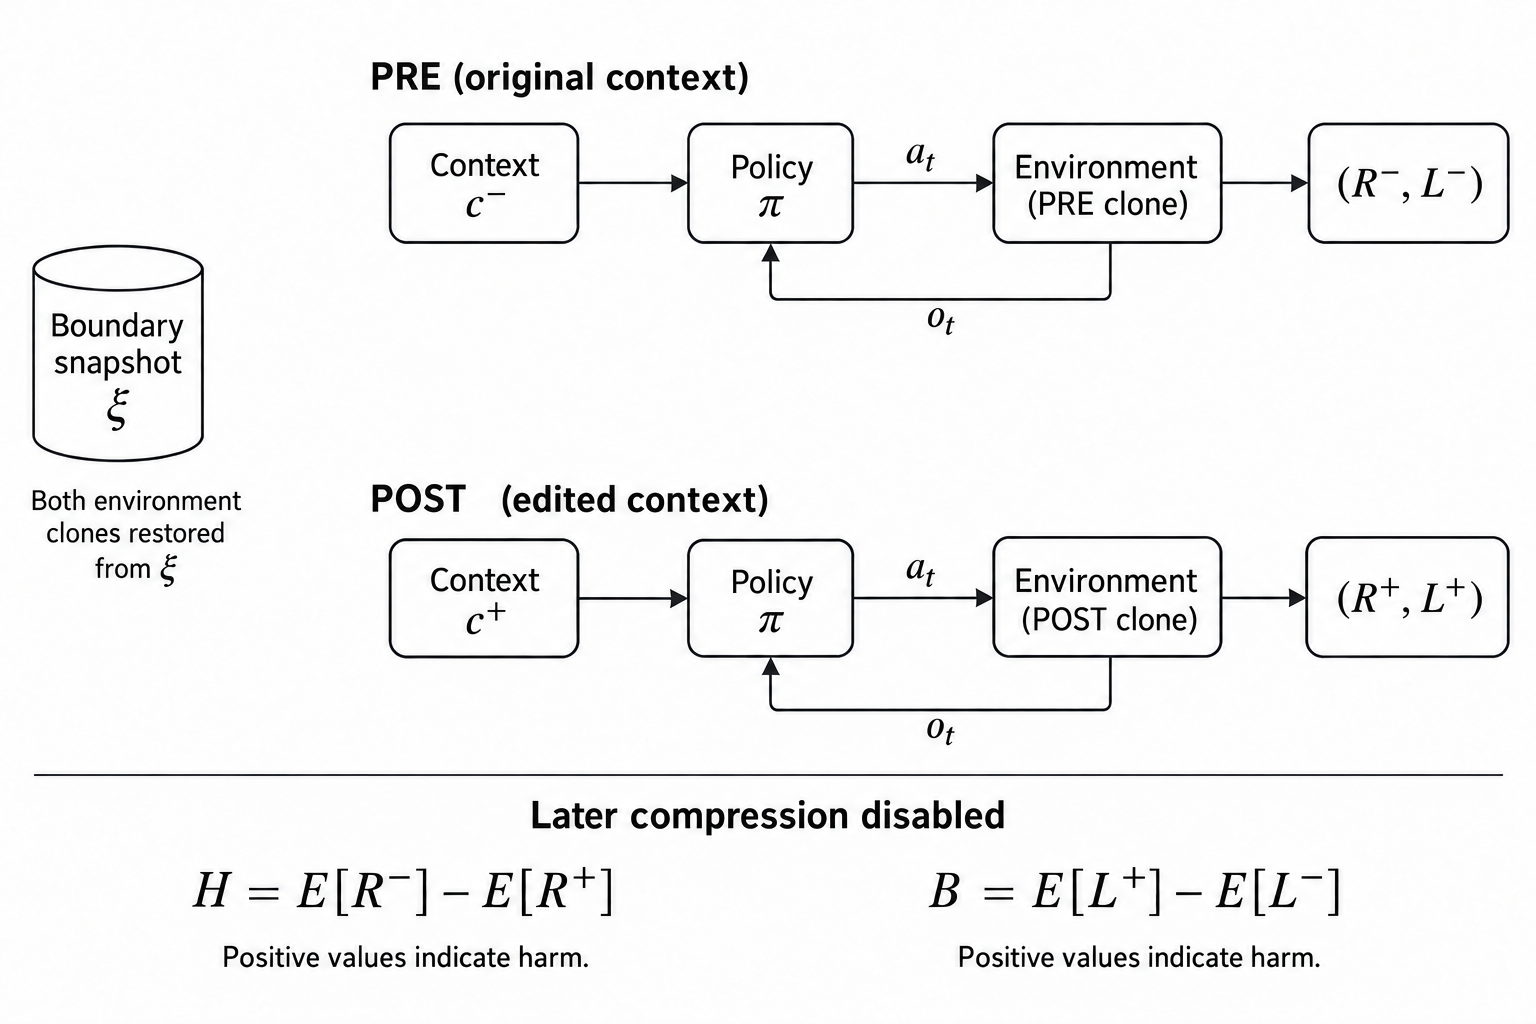
\includegraphics[width=\linewidth]{book/figures/assets/F12review.png}
\caption{A paired continuation diagnostic changes the working view while restoring the same external boundary state and holding the continuation policy fixed. Disabling later compression isolates the current replacement. Outcome hazard $H=\mathbb E[R^-]-\mathbb E[R^+]$ and interaction burden $B=\mathbb E[L^+]-\mathbb E[L^-]$ quantify different consequences. Estimation requires validated restoration and repeated continuations; no outcomes are depicted. Original schematic informed by PAIR~\cite{min2026pair}.}
\label{fig:C12:paired-context-intervention}
\end{figure}

\section{Editing and cache validity}\label{sec:C12:cache}
Text editing changes the input sequence, while cache reuse assumes particular computational dependencies remain valid. In a standard causal transformer, a cached hidden state for a later token can depend on earlier tokens through attention and residual computation. Deleting an earlier span does not generally leave later states unchanged, even if the surviving text is byte-identical. Reusing cached values therefore requires a justified dependency rule, not merely matching the visible suffix.

For a simple prefix-cache implementation, an edit at position $j$ invalidates the reusable prefix from that position onward. If $L$ is the new length, the re-prefill work depends on $L-j$ as well as newly generated tokens. A context policy that repeatedly edits early content can reduce token count while destroying reuse. This explains why a representation optimized only for shortness can be expensive under an actual serving architecture. The relevant objective includes both retained size and edit location.

PagedAttention addresses logical and physical allocation and sharing of cached blocks~\cite{kwon2023pagedattention}. It does not, by itself, establish that arbitrary semantic edits preserve the numerical validity of a cached block. A page allocator may retain bytes correctly while the model computation those bytes represent is no longer appropriate for the edited sequence. Allocation validity and inference validity must be checked separately.

CLM Suffix Cache Reuse is an explicit approximation: surviving suffix states retain dependencies on the pre-edit prefix~\cite{shao2026context}. Its full-attention path re-rotates relocated keys for their new positions, while the studied hybrid path resumes pre-edit recurrent state instead of recomputing inserted content in linear-attention layers. Position adjustment does not remove stale content dependencies. Report this quality--compute tradeoff separately from exact prefix reuse and from measured end-to-end latency.

An edit-aware serving contract can attach a dependency fingerprint to every reusable region. The fingerprint identifies model version, tokenizer, position convention, attention mask, and relevant predecessor state. A reuse decision is valid only if the implementation's equivalence conditions hold. Exact fingerprints may be expensive; conservative invalidation sacrifices reuse to preserve correctness. Approximate reuse is possible, but its approximation should be evaluated as a quality tradeoff rather than described as lossless without proof.

Measure context-control latency end to end. Include the editing model call, storage writes, cache invalidation, re-prefill, extra retrieval, and any retries after a damaged summary. Report warm and cold behavior separately. A policy that looks strong when every prompt receives a fresh prefill can perform differently in a service with extensive prefix reuse. The comparison must reflect the intended deployment instead of selecting the serving regime most favorable to one method.


\section{A worked decision-preservation analysis}\label{sec:C12:worked}
Consider a task with three obligations: modify a parser, preserve a legacy behavior, and produce a reviewable patch without publishing it. The raw history includes a failed test, a revised hypothesis, and a user correction that narrows the authorized output. A token-oriented summarizer may retain the patch plan and the latest test output while dropping the legacy requirement and the authorization correction as old discussion. The resulting input is shorter but misrepresents the permitted output scope and success requirements in the model-visible view.

Represent the validated state as $z=(G,O,A,E,U)$: goals $G$, obligations $O$, authority $A$, evidence references $E$, and unresolved hypotheses $U$. A proposed compaction operator $T$ should preserve $O$ and $A$ exactly, preserve enough of $E$ to justify current conclusions, and mark unresolved hypotheses as unresolved. This is an application-specific contract. It does not claim that these five fields are sufficient for every task; it states which distinctions this parser workflow requires.

Suppose the original and compacted policies induce action distributions $p$ and $q$ at the next decision. For a bounded immediate loss $0\leq\ell\leq1$, their expected losses differ by at most $\mathrm{TV}(p,q)$. If a validator can establish a bound on distribution change, that bound controls immediate risk under the stated loss. It does not automatically control the complete task, because a small action change can place the environment in a different region. Long-horizon guarantees require bounds on transition sensitivity or repeated coupling assumptions, which are rarely available for arbitrary tools.

For deterministic safety constraints, comparing distributions is unnecessary. Suppose every tool call passes the same monitor, whose allowed-action set is determined exclusively by the authoritative grant state and the current enforcement configuration. Holding those inputs fixed preserves the same syntactic boundary even when compaction changes the policy. Copying an old $A$ into a summary does not satisfy this condition after a grant is revoked; the monitor must consult current authority at dispatch, independently of the edited prose. Semantic correctness remains open: the agent can take an allowed but wrong action. This separation is valuable because it prevents summary quality from being responsible for all enforcement. Authority should survive in a typed control layer even when task evidence is compressed.

The corresponding experiment compares four views: full history, generic summary, typed-state summary, and typed state plus targeted raw retrieval. Keep the model, tools, and environment snapshot fixed. Randomize whether the legacy constraint appears early or late and whether the latest correction expands or narrows authority. Score patch correctness, publication behavior, retrieval use, and cost separately. This is a proposed experiment. No numerical outcomes are implied by the formulation.

A successful typed-state condition would support the mechanism that explicit obligations survive compression in this workload. It would not establish that a manually designed schema generalizes to unknown scientific or legal tasks. A failure would still be useful if it identifies a missing state field or an incorrect validation rule. The scientific objective is to expose which information transformations preserve behavior, rather than to award a generic summary the label of memory.


\section{Evidence comparisons and causal boundaries}\label{sec:C12:evidence}
ContextPilot separates the editing toolset from the learning rule. Its tools include structured memory, notes, planning, and reversible context offload. Training uses snapshots at editing boundaries, masks previously optimized tokens, and allocates continuation sampling around consequential editing actions~\cite{pan2026contextpilot}. Its action-level feedback addresses the fact that final task correctness is an imperfect label for every earlier edit. This does not make the feedback causal ground truth: continuation outcomes still depend on the downstream policy and environment. A comparison must separate the expanded toolset, supervised initialization, branch allocation, and advantage estimator rather than attributing their joint effect to one component.

CompactionRL jointly trains execution and summary generation with token-level normalization. Its cross-segment credit correction is approximate, not exact full-trajectory GAE~\cite{li2026compactionrl}. For segment $s$ with $n_s\geq1$ optimized tokens, discount $\gamma\in(0,1]$ and trace parameter $\lambda\in(0,1]$, the method scales its locally computed advantages by the number of later optimized tokens:
\begin{equation}
 \widehat A_{s,i}=(\gamma\lambda)^{N_{>s}}A^{\mathrm{loc}}_{s,i},
 \qquad N_{>s}=\sum_{j>s}n_j.
 \label{eq:C12:compactionrl-position}
\end{equation}
This restores the terminal-reward discount distance when the shared reward is placed at each independently optimized segment end. It does not recursively propagate all later TD residuals into earlier segments. The authors trade that reconstruction for parallel segment processing; a reproduction must distinguish reward-distance correction from full-trajectory GAE. Their coding evaluation uses a specified 200-task SWE-bench Verified subset, rather than the full benchmark. Successful joint optimization does not establish preservation of arbitrary future constraints.

TRACE v2 evaluates candidate summaries through paired closed-loop continuations from the same AppWorld state while keeping the agent and proposer weights frozen~\cite{cumulative_a_trace_v2_20261029}. Its local verifier counts the union of blocked actions and canonicalized repeated tool calls over a fixed horizon; this does not detect every silent state corruption. Preferences between summaries reuse the same PRE continuations. The proposer receives the downstream system prompt, compressor input, and better--worse summary pairs, but not rollout traces or the verifier decomposition. Five candidate compression templates are then selected on development-set success in both repeated runs, not success in either run; the selected template is frozen for test evaluation. This separates boundary-local supervision, prompt selection, and held-out testing. The evidence remains concentrated in AppWorld, and restoration fidelity and verifier scope limit the causal interpretation.

PAIR likewise uses counterfactual continuations to identify damaging individual compressions and adapts sections of a structured prompt~\cite{min2026pair}. It distinguishes repeated-run reliability from finding one successful attempt. Its offline continuation search and restored-state access are part of the adaptation cost. These requirements can be reasonable in an experimental environment while unavailable for an external business tool with irreversible side effects. TRACE and PAIR share research lineage, so their agreement is evidence of a developing mechanism rather than two independent replications.

These mechanisms expose a concrete disagreement with purely semantic compression objectives. A summary can retain entities and facts yet obscure whether an action already happened, whether a plan is obsolete, or whether the task is complete. In that case the failure is execution-state mislocalization, not necessarily absence of a fact. Evaluating summary similarity would miss the directional role of action-observation history. The appropriate response is to preserve validated progress and effect receipts, then test whether the agent stops, resumes, and avoids repeating completed work. This is a synthesis of the mechanisms above, not a new measured result.

ACM provides author-reported evidence that explicit context actions can improve its evaluated tasks while reducing peak active context~\cite{corpus260723809}. The same study also illustrates why resource metrics must remain separate: in its reported BrowseComp-Plus comparison, tool calls increase from 19.5 to 46.2 per episode. This observation does not negate a context benefit; it limits the inference that smaller context necessarily means lower total latency or expense. These results have not been independently reproduced for this monograph.

Comparing learned compaction with deterministic summarization requires matching more than model identity. A learned controller may have seen environment-specific trajectories, received a larger training budget, or benefited from a retriever tuned to the evaluation interface. An ablation that removes the controller but also removes access to raw history changes two mechanisms simultaneously. Preserve the same storage and retrieval interfaces while varying the decision policy if the claim concerns control rather than memory availability.

Author-reported improvements across several benchmarks can support broader relevance, but shared infrastructure creates dependence between results. The same backbone, tool wrapper, answer extraction, and evaluator may appear across tasks. A cross-domain average does not turn those results into independent replications. Report task-specific outcomes and explain which components are shared. If one task improves and another regresses, the average should not hide the mechanism-specific disagreement.

The key comparison axes are behavior preservation, resource accounting, reversibility, training consistency, and implementation transparency. Full-history methods preserve observations but can suffer distraction and expense. Summaries reduce active input but can lose qualifications. Retrieval retains scalable access but can miss implicit relevance. Editable contexts increase flexibility but complicate cache and rollout semantics. These are structural tradeoffs, not a ranking without workload assumptions.

Evidence should also identify what remains unavailable. If a paper describes prompts but releases no execution adapter, code-level reproduction is incomplete. If code exists but requires a private checkpoint or undisclosed environment, the visible repository does not close that gap. A reproducibility claim should identify model weights, data, tool fixtures, edit policy, and evaluation version. Successful compilation of a harness is not successful reproduction of its scientific results.

The practical implication is to choose the simplest context-control mechanism that satisfies measured task and authority constraints. A sophisticated learned editor can be appropriate when decision value changes rapidly and enough training feedback exists. A deterministic structured state can be preferable when obligations are explicit and failures are costly. The evidence needed to choose between them is a matched workload study, not the elegance of the editing interface.

An October 2026 alternative is transparent-compact for the Pi coding agent. The inspected paper evaluates version 0.8.0, retaining user messages and assistant prose verbatim while masking tool outputs and reasoning, explicitly marking removed material, and providing delegated recovery~\cite{woolford2026transparent}. Its recovery action is \path{context_lookup}, with bounded fallback access. The guarantees are budget-limited: when retained prose reaches the configured cap, truncation begins. It therefore does not establish indefinite verbatim memory. Its next-turn probes concern commitments and planted facts with file and shell tools removed to isolate conversational memory. They do not establish complete software-engineering task success.

This method exposes a different comparison axis from learned abstraction. It preserves what was said while declining to treat that prose as verified truth. A retained assistant claim can still be wrong, and a removed tool result can require recovery before the claim is reused. The working view gains transparency about missing evidence at the cost of carrying more conversational text. Whether that tradeoff improves a task depends on the importance of exact commitments, the recoverability of observations, and the model's tendency to act confidently on an ambiguous summary.

The pinned CLM implementation supplies a concrete interface boundary. In \path{clm/clm_harness/context_env/env.py}, \path{ContextEnv._apply_edit} round-trips candidate messages through \path{parse_back}, counts tokens, and invokes \path{edit_gate.may_grow} before replacement~\cite{repo_clm2026}. The gate constrains growth; a shrinking edit that remains over budget can still be accepted with a warning, so this helper alone is not an absolute budget-admission guard. In \path{clm/clm_harness/context_utils/context_string.py}, \path{parse_back} restores the protected prefix but maps every editable non-assistant role to user text and does not reconstruct structured tool calls. Legal serialization therefore does not preserve all original role and effect provenance. Evaluate those changes separately from semantic commitment preservation and from the stricter proposed admission contract in Eq.~\eqref{eq:C12:context-admissibility}.

\section{Failure recovery and implementation discipline}\label{sec:C12:recovery}
Context transformations should be recoverable operations. Persist the source view and its edit manifest before replacing the active context. Commit the replacement only after structural validation, and retain a rollback reference until the affected task stage has been verified. This does not require keeping every cache allocation forever; it requires retaining enough evidence and metadata to reconstruct the decision input. Storage retention and privacy constraints still apply.

Use separate error classes for failed summarization, invalid serialization, missing raw evidence, retrieval failure, and an edited view that violates a pinned obligation. A generic ``context error'' obscures whether the model, controller, or storage layer is responsible. Recovery can then be targeted: restore the prior view, fetch an omitted record, regenerate an abstraction, or stop before a consequential tool effect. Blindly retrying the same damaged summary can amplify the failure.

Concurrent editing requires ownership. If a worker updates a plan while a controller compacts an older version, a last-write-wins replacement can erase legitimate progress. An optimistic commit should compare the base view version with the current version and reject or merge a stale edit. Semantic merges deserve special treatment: two summaries can each be locally valid while their union contains contradictory commitments. A storage-level conflict resolution rule cannot determine which commitment the user currently authorizes.

Human-readable state remains useful for audit, but readability should not replace machine-checkable boundaries. Identifiers, timestamps, tool-effect receipts, authority, and completion predicates can be represented in typed fields. Generated prose can explain those fields without becoming their sole source of truth. The boundary between recorded fact and model inference should survive every compaction. This reduces the chance that repeated summaries gradually promote a tentative hypothesis into an asserted observation.

The implementation path is incremental. First instrument the existing context assembly. Then introduce explicit source references and pinned obligations. Next add reversible offload with deterministic triggers. Only after those controls are measurable should a learned editing policy be compared under matched budgets. This sequence is a systems deduction about observability and attribution, not a claim that one particular product follows it or that it guarantees success.

The strongest outcome of context engineering is not a permanently small prompt. It is a working view whose contents, omissions, cost, and authority are deliberate and inspectable. Such a view supports the policy's current decisions while preserving a path back to evidence when assumptions change. Durable sessions in Chapter~\ref{ch:C13} provide the substrate for that path; persistent memory in Chapter~\ref{ch:C14} determines which evidence and abstractions remain useful across tasks.

